This section introduces the AGREE contract specification language through the cyber-hardened system of \figref{fig:hardened}.
It details the specification of that top-level system interface.
It then discusses the specifications for the filter and the monitor added by the transforms.

This section then formalizes AGREE's assume-guarantee reasoning by defining the set of verification conditions that AGREE must check.
The verification conditions succinctly summarize what in means when AGREE proves that a system implementation satisfies it specification.
These conditions are useful in understanding how the semantics in synthesis differ from those in the assume-guarantee reasoning in \secref{sec:semantics}.

\subsection{Contract Specification}
\newsavebox{\sw}
\begin{lrbox}{\sw}
\begin{lstlisting}[style=agree,numbers=left]
eq req : bool = event(AutomationRequest);
eq avl : bool = event(AirVehicleLocation);
eq wp : bool = event(Waypoint);
eq strt: bool = event(Start);
eq alrt : bool = event(Alert);

assume "Automation requests are well-formed" :
  req => WELL_FORMED_AUTOMATION_REQUEST(AutomationRequest);
assume "Air vehicle locations are well-formed" :
  avl => WELL_FORMED_WAYPOINT(AirVehicleLocation);    
assume "One automation request in flight at a time" :
  true -> 
  (req => pre(Historically(not req) or Since(not req, strt)));
      
guarantee "Waypoints coincide with air vehicle locations":
  wp => avl;
guarantee "Starts include a new waypoint" :
  strt => wp;
guarantee "Waypoints are well-formed" : 
  wp => WELL_FORMED_WAYPOINT(Waypoint);
guarantee "Starts within one cycle of requests if not alerting" :
  (strt => ((not alrt) and req)) -> 
  (strt => ((not alrt) and (req or pre(req))));
guarantee "Alert if not started within one cycle of requests" :
    true -> ((pre(req and not strt) and not strt) => alrt);
guarantee "Once alerted always alerted" :
  not alrt or (Once(alrt) and alrt);
\end{lstlisting}
\end{lrbox}

\begin{figure}
  \begin{center}
    \scalebox{0.62}{\usebox{\sw}}
  \end{center}
  \caption{The SW component contract.}
  \label{fig:sw}
\end{figure}

The AGREE specification for the SW component in the example of Section~\ref{sec:example} with the added cyber requirements is given in \figref{fig:sw}.
The AGREE specification language is a first-order predicate calculus that uses stream concepts, and operators, from the Lustre language \cite{10.1145/41625.41641}.
As with Lustre, the semantics are synchronous dataflow where the inputs, outputs, and expressions are data streams that comply with the input assumptions.
Contracts are evaluated in dependency order with inputs being propagated to outputs through all contracts until they stabilize; as such, the contracts, and thereby the top-level model, must be acyclic.\footnote{An apparent syntactic cycle, where a component is linked back to itself, may be broken temporally by inserting delay elements.}
Once the contracts have stabilized, the model takes a synchronous step to the next input data in the stream.
The semantics do not model computation or communication delay.
The output of one contract is seen at the input of any downstream contract in the same step of the input data stream.

The AGREE model checker attempts to prove several properties of the top-level model being verified.
The first is that the output guarantees of each component implementing the system are strong enough to validate the input assumptions of any downstream component as well as to satisfy the guarantees of the output of the top-level component being verified (\ie, the system composition meets input assumptions at each input as well as the guarantees on the system output).
These properties are reported in the expanded lists in \figref{fig:example}(b) and \figref{fig:hardened}(b).
The next set of properties prove that the contract specifications for each component are \emph{self-consistent} \ie, a contract does not contradict itself.
These are the unexpanded results at the bottom of the figures.

Returning back to the contract of \figref{fig:sw}, it uses \texttt{eq} statements to define variables local to the contract specification.
For example, the \texttt{req} variable is equivalent to the \texttt{event(AutomationRequest)} expression.
In the AGREE semantics, there is an implicit \emph{event} input (or output) associated with every named event port in a component.
The semantics used here do not buffer these events so the implicit input (or output) is only a boolean value.
An \texttt{event} expression refers to that implicit input (or output) and is true when data is placed on the named port.
The system contract here states assumptions on well-formed input, followed by guarantees on properties about the output.

REPLACE ALL: 
The \emph{Alert if start is not bounded relative to a request} guarantee is an invariant on the expression \texttt{policy or since}, meaning that either the policy holds or the alert is sounding.
The \texttt{policy} is defined by two local values: \texttt{current} and \texttt{previous}.
The \texttt{current} value is asserted when in the current time step there is a request with a response, or there is no request and no response.

The value of \texttt{previous} in the current time step relies on values from the previous time step.
The \texttt{->} operator designates initialization, as the previous time step is undefined in the first step of the system.
The left operand to the operator is the initial value of \texttt{previous} at start, which in this example is \texttt{(req and not rsp)}, because seeing a request with no response is inconclusive in the first step of the system.
The right operand is the value of \texttt{previous} after the initial step.
Here the \texttt{pre} operator refers to the value of the expression \texttt{(req and not rsp)} in the prior time step, \texttt{previous} is true if the previous time step made a request without a matching response and the current time step has the matching response to that request with no new request.

The value of \texttt{since} in \emph{Alert if start is not bounded relative to a request} relies on its own value in the previous time step.
The intuitive reading of the expression is that the alert has been true since the time when it first sounded.
The first \texttt{alrt} sets \texttt{since} to true, and once the value of \texttt{since} is true, that value persists as long as \texttt{alrt} holds.
The \emph{Alert if start is not bounded relative to a request} guarantee defines one requirement of a cyber-hardened system implementation.
Together with the other guarantees, the contract models the expected input and output of the system as a whole.

\begin{figure}
  \begin{center}
    \begin{tabular}{c}
      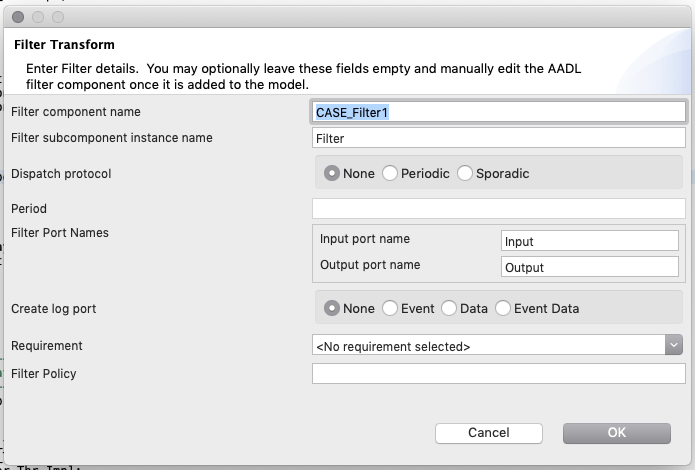
\includegraphics[scale=0.3]{dialogue.png}
    \end{tabular}
  \end{center}
  \caption{Wizard for automatically transforming the model with a filter.}
  \label{fig:dialogue}
\end{figure}

\newsavebox{\flt}
\begin{lrbox}{\flt}
\begin{lstlisting}[style=agree,numbers=left]
eq policy : bool = 
  WELL_FORMED_AUTOMATION_RESPONSE(Input);

guarantee Filter_Output
  "Filter output is well-formed" :
  if event(Input) and policy then 
    event(Output) and Output = Input
  else not event(Output);
\end{lstlisting}
\end{lrbox}

\newsavebox{\mntr}
\begin{lrbox}{\mntr}
\begin{lstlisting}[style=agree,numbers=left]
const is_latched : bool = true;
const MAX_LATENCY : int = 1;
    
eq rsp : bool = event(Response);
eq req : bool = event(Request);

eq isPending : bool = Since(not rsp, req and not rsp);
eq latency : int = 0 -> (if req then 0 else pre(latency) + 1);

eq policy : bool = (rsp => req) ->
                   (    (isPending => latency < MAX_LATENCY)   
                    and (rsp => (req or pre(isPending))));
eq alert : bool = (not policy) -> 
                  ((is_latched and pre(alert)) or not policy);

assume "One outstanding request at a time" :
  (true -> (req => not pre(isPending))); 
                          
guarantee "Alert port tracks alert variable" :
  event(Alert) = alert;
guarantee "Output if not alerted" :
  if (not(alert) and rsp) then
    event(Output) and (Output = Response)
  else
    not (event(Output));    
\end{lstlisting}
\end{lrbox}

\begin{figure}
  \begin{center}
    \begin{tabular}{c}
      \scalebox{0.62}{\usebox{\flt}} \\
    \end{tabular}
  \end{center}
  \caption{Contract specification for high-assurance filter.}
  \label{fig:filter}
\end{figure}

\begin{figure}
  \begin{center}
    \begin{tabular}{c}
      \scalebox{0.62}{\usebox{\mntr}} \\
    \end{tabular}
  \end{center}
  \caption{Contract specification for high-assurance monitor.}
  \label{fig:monitor}
\end{figure}

As noted previously, the original system fails to guarantee the cyber requirements.
BriefCASE provides two transformations to address the failing requirements: inserting a filter and inserting a monitor.
The component is added by selecting the connection in the model where the high-assurance component is to be added, and then choosing the appropriate transformation.
The system designer can provide transform configuration parameters in a wizard, as shown in \figref{fig:dialogue}.
The policy of the high-assurance component can be stated directly in the wizard, or it can be left blank.
In this example, the policy is specified as \texttt{WELL\_FORMED\_AUTOMATION\_RESPONSE(Input)}.
Additionally, because a transformation is ultimately driven by a cyber requirement, BriefCASE updates an embedded Resolute assurance case~\cite{resolute-destion}.
REMOVE: Resolute keeps track of the evidential artifacts necessary for supporting the requirement, and can be run at any time to determine whether those artifacts are valid.

The AGREE contract specification generated by the transform is shown in \figref{fig:filter}.
The guarantee is stylized for synthesis and completely defines the meaning of the output under every possible input.
The resulting AGREE specification for the monitor in this example is shown in \figref{fig:monitor}.
The \texttt{is\_latched} value makes the alert persistent, meaning that once the alert is raised, it is always raised.
This behavior is one of the several options available in the dialogue.
The definition for \texttt{policy} is taken by the system developer from the contract in \figref{fig:sw}.
As before, the guarantees for the outputs are autogenerated by the tool and completely define each output under every possible input.

\subsection{Verification Conditions}

\newcommand{\globally}{\ensuremath{\mathbf{G}}}
\newcommand{\historically}{\ensuremath{\mathbf{H}}}
\newcommand{\assumes}{\ensuremath{A}}
\newcommand{\guarantees}{\ensuremath{P}}
\newcommand{\dispatch}{\ensuremath{\mathit{dispatch}}}
\newcommand{\complete}{\ensuremath{\mathit{complete}}}
\newcommand{\same}[1]{\ensuremath{\mathit{same}(#1)}}
\newcommand{\inputs}{\ensuremath{I}}
\newcommand{\outputs}{\ensuremath{O}}
\newcommand{\system}{\ensuremath{S}}
\newcommand{\components}{\ensuremath{C}}
\newcommand{\component}{\ensuremath{c}}
\newcommand{\schedule}{\ensuremath{\phi}}
\newcommand{\valid}{\ensuremath{\mathit{valid}}}
\newcommand{\dpred}{\ensuremath{\delta^\phi}}
\newcommand{\dispred}{\ensuremath{\mathbb{D}^\phi}}
\newcommand{\compred}{\ensuremath{\mathbb{C}^\phi}}
\newcommand{\dispredp}{\ensuremath{\mathbb{D}^{\phi\prime}}}
\newcommand{\compredp}{\ensuremath{\mathbb{C}^{\phi\prime}}}

The AGREE specification language is based on stream concepts, and
operators, from the Lustre language \cite{10.1145/41625.41641}. Thus
the setting is synchronous dataflow where the inputs and outputs of
components are streams, and contracts express relationships between
input and output streams. When considering a system of components,
data flows through the components in dependency order, with inputs
being propagated to outputs through all contracts until they stabilize
(can't propagate further). Therefore, the subcomponent contracts, and
thus the top-level model, must be acyclic. (An apparent syntactic
cycle, where a component is linked back to itself, may be broken
temporally by inserting delay elements.)  Once the data propagation
has stabilized, the model proceeds to the next input data in the input
streams. The semantics do not model computation or communication
delay. The output of one contract is seen at the input of any
downstream contract in the same step of the input data stream.

From the system and component contracts, AGREE generates a set of
verification conditions to show that a system's component
implementation is correct~\cite{agree2013}.  The AGREE model checker
is then invoked to prove or disprove the verification
conditions. Contracts and verification conditions are expressed in
\emph{past-time linear temporal logic} (PLTL).\footnote{KLS: citation
needed.}  PLTL is a logic enhanced with temporal operators able to
reason about the truth values of formulas through time.  Its semantics
are defined relative to a point in time $i$ and a finite trace of
system states $\pi = s_0, s_1, \ldots, s_i$.

The two PLTL operators necessary for the AGREE generated verification
conditions are $\globally$ (globally) that looks forward in time along
the trace and $\historically$ (historically) that looks backward in
time along the trace.  These are defined as
\begin{eqnarray*}
 (\pi, i) \models \globally(f) & \iff & \forall j \ge i, (\pi, j) \models f \\
(\pi, i) \models \historically(f) & \iff & \forall 0 \le j \le i, (\pi, j) \models f
\end{eqnarray*}
The $\models$-operator is read as \emph{satisfies}.  A trace at a
moment in time satisfies $\globally(f)$ if and only if it satisfies
$f$ in the current and all future states of $\pi$.  $\globally(f)$ is
invariant from the current moment into the future and $\historically$ is
invariant from the beginning of the trace to the current moment.

A \emph{system} $\system = (\inputs, \outputs, \assumes,
\guarantees,C)$, where $\inputs$ is the input set, $\outputs$ is the
output set, $\assumes$ is the set of assumptions, $\guarantees$ is the
set of guarantees, and $C$ are subcomponents.  A subcomponent
$\component$ is, hierarchically, also a system, and may be designated
by its own tuple $(\inputs_\component, \outputs_\component,
\assumes_\component, \guarantees_\component, C_c)$.  From the
components and their connections, $\mathbb{I}_\component$ is defined
to be the set of components providing input to some component
$\component$ in the system, and $\mathbb{O}$ is defined to be the set
of components that provide the output for the system.  A system $S$ is
\emph{correct} if and only if for all components $c \in C$ the
following two verification conditions hold:
\begin{equation}
            \globally(\historically(\assumes \wedge
            \bigwedge_{\component^\prime \in \mathbb{I}_\component} P_{\component^\prime})
            \implies \assumes_\component)
\end{equation}
\begin{equation}
            \globally(\historically(\assumes \wedge
            \bigwedge_{\component^\prime \in \mathbb{O}} \guarantees_{\component^\prime})
            \implies \guarantees)
\end{equation}
Condition (1) verifies the input assumptions on each component under
the system assumptions and upstream component guarantees.  It checks
if the component guarantees and system assumptions are strong enough
to imply input assumptions on all immediate downstream components.
Condition (2) checks the output guarantees of the system under the
system assumptions and component guarantees that provide the output.
It checks if the guarantees on components providing primary outputs
are strong enough to imply the system guarantees.

If all the verification conditions hold (AGREE uses $k$-inductive
model checking to automatically prove or disprove each generated
verification condition), then the system is said to be \emph{correct},
meaning that the system composition meets input assumptions at each
input as well as the guarantees on the system output. A consequence of
this result is that $\globally(\historically(\assumes) \implies
\guarantees)$ holds for the system contract.

The expanded property lists in \figref{fig:example-certificate} and
\figref{fig:hardened-certificate} are the results from verifying or
disproving the above verification conditions.  The additional
unexpanded results at the bottom of the figures prove
\emph{self-consistency} in the contracts.  It is not uncommon to
accidentally write contracts that are self-contradicting.  For
example, a contract may guarantee an output be two different values in
the same moment of time.  AGREE generates additional verification
conditions that prove each component contract, and the composition of
contracts, self-consistent.

